% -----------------------------------------------------------------
%  main.tex –  Plantilla con modo Equipo / Individual
% -----------------------------------------------------------------
\documentclass[letterpaper,12pt]{article}

% ----------------------  Paquetes base ---------------------------
\usepackage[utf8]{inputenc}
\usepackage[T1]{fontenc}
\usepackage{lmodern}
\usepackage[spanish,mexico]{babel}
\usepackage{amsmath,amssymb,amsfonts}
\usepackage{array,booktabs}
\usepackage{graphicx}
\usepackage{float}
\usepackage{fancyhdr}
\usepackage{hyperref}
\usepackage[square,numbers]{natbib}
\usepackage{parskip}
\usepackage{xcolor}
\usepackage{datetime2}
\usepackage{draftwatermark}
\usepackage{algorithm}
\usepackage{algpseudocode}
\usepackage{listings}
\usepackage[shortlabels]{enumitem}
\usepackage[normalem]{ulem}  
\usepackage{ifthen}
\usepackage{etoolbox} 
\usepackage{tikz}
\usetikzlibrary{shapes.geometric, arrows.meta, positioning}
\DeclareUnicodeCharacter{202F}{\,}

% -------------------  Macros para integrantes --------------------
% Integrante:  #1 Nombre  #2 Matrícula  #3 Hora  #4 OK/OUT
\newcommand{\Integrante}[4]{%
	\ifthenelse{\equal{#4}{OUT}}%
	{\textcolor{red}{\sout{#1}} & \textcolor{red}{\sout{#2}} & \textcolor{red}{\sout{#3}} \\}%
	{#1 & #2 & #3 \\}%
}
\newcommand{\ListaIntegrantes}{}   % se redefine en datos.tex

% --------------  Macros para entrega individual ------------------
\newcommand{\SingleName}{}  % Nombre del alumno
\newcommand{\SingleMat}{}   % Matrícula
\newcommand{\SingleHora}{}  % Hora clase
\newcommand{\EntregaIndividual}{false} % "true" o "false" (datos.tex)

% --------------------  Configuración general ---------------------
\hypersetup{colorlinks=true, linkcolor=blue, urlcolor=blue}
\lstset{basicstyle=\ttfamily\footnotesize, numbers=left,
	frame=single, breaklines=true, tabsize=2, captionpos=b}

% Cargar datos específicos
% -----------------------------------------------------------------
%  datos.tex – Metadatos de portada para la Actividad Fundamental 3
% -----------------------------------------------------------------
\newcommand{\myMateria}{Introducción a la Inteligencia Artificial}
\newcommand{\myGrupo}{001}
\newcommand{\myTeam}{1}
\newcommand{\MyReport}{Aplicación de Clustering No Supervisado (K-Means) para la Estratificación de Perfiles Clínicos de Riesgo Cerebrovascular}
\newcommand{\myUnidad}{Actividad Fundamental 3 — Introducción al Aprendizaje Máquina}
\newcommand{\myDate}{20/11/2026}
\newcommand{\myTeacher}{Por confirmar}
\newcommand{\myHora}{Lunes, Miércoles y Viernes — V2}

% -------- Modo de entrega ----------------------------------------
% "false" = trabajo en equipo (tabla)   |   "true" = trabajo individual
\renewcommand{\EntregaIndividual}{false}

% -------- Lista de integrantes (solo para modo equipo) -----------
\renewcommand{\ListaIntegrantes}{%
	\Integrante{Butzmann Martinez Sergio Jaziel}{2163239}{V2}{OK}
	\Integrante{Diego Carrillo Castillo}{2144556}{V2}{OK}
	\Integrante{Uriel Samuel Bravo Castillo}{2227015}{V2}{OK}
	\Integrante{Gustavo Guzman Puente}{Por confirmar}{V2}{OK}
	\Integrante{Vanessa Rodriguez Colunga}{2158341}{V2}{OK}
}

% -------- Datos individuales (si EntregaIndividual = true) -------
\renewcommand{\SingleName}{Butzmann Martinez Sergio Jaziel}
\renewcommand{\SingleMat}{2163239}
\renewcommand{\SingleHora}{V2}


% Marca de agua
\newcommand{\WatermarkText}{}
\ifthenelse{\equal{\EntregaIndividual}{false}}{%
	% Equipo
	\renewcommand{\WatermarkText}{Grupo \myGrupo\ – Equipo \myTeam\ — \DTMnow}%
}{%
	% Individual
	\renewcommand{\WatermarkText}{\SingleName\ (\SingleMat)\ — \DTMnow}%
}

\SetWatermarkText{\textsc{\WatermarkText}}
\SetWatermarkScale{0.15}
\DraftwatermarkOptions{color={[RGB]{235,235,235}}, angle=55}

% Márgenes y encabezado
\textheight=22cm \textwidth=17cm
\topmargin=-1.6cm \oddsidemargin=-0.3cm
\fancyhf{}
\lhead{\myMateria}
\rhead{\myUnidad}
\fancyfoot[C]{\thepage}
\rfoot{\DTMnow}
\setlength{\headheight}{33pt}
\pagestyle{fancy}

% -------------------------- Documento ----------------------------
\begin{document}
	
	\thispagestyle{empty}

% Escudos ----------------------------------------------------------
\begin{figure}[ht]
	\minipage{0.4\textwidth}\centering
	
\includegraphics[width=3cm]{Imágenes/FIME_LOGO}
	\endminipage\hfill
	\minipage{0.4\textwidth}\centering
	
\includegraphics[width=3cm]{Imágenes/logo_uanl}
	\endminipage
\end{figure}

\vspace{0cm}

% Encabezado institucional ----------------------------------------
\begin{center}
	{\large\scshape Facultad de Ingeniería Mecánica y Eléctrica\par}
	{\normalsize\scshape Universidad Autónoma de Nuevo León\par}
	\vspace{0.5cm}
	{\Large\textbf{\myMateria}\par}
	\vspace{0.25cm}
	{\LARGE\textbf{\MyReport}\par}
	\vspace{0.2cm}
	{\Large \myUnidad\par}
	\vspace{0.5cm}
	{\large\textbf{Fecha:} \myDate\par}
	\vspace{0.2cm}
	{\large\textbf{Día y hora de clase:} \myHora \quad | \quad \textbf{Grupo:} \myGrupo\par}
	\vspace{0.2cm}
	{\large\textbf{Profesor:} \myTeacher\par}
	\vspace{0.6cm}

	% ---------- Tabla o bloque individual según bandera --------------
	\ifthenelse{\equal{\EntregaIndividual}{false}}{% -------------- EQUIPO
		{\large\textbf{Integrantes (Equipo \myTeam)}\par}
		\vspace{0.3cm}
		\renewcommand{\arraystretch}{1.15}
		\begin{tabular}{p{8cm} p{3cm} p{2cm}}
			\textbf{Nombre} & \textbf{Matrícula} & \textbf{Hora} \\ \midrule
			\ListaIntegrantes
		\end{tabular}
	}{% -------------------------------------------------- INDIVIDUAL
		{\large\textbf{Datos del alumno}\par}
		\vspace{0.3cm}
		\textbf{Nombre:} \SingleName \\[2pt]
		\textbf{Matrícula:} \SingleMat \\[2pt]
		\textbf{Hora clase:} \SingleHora
	}
\end{center}

\clearpage

	
	\tableofcontents
	\newpage
	
	% =================================================================
%  contenido.tex – Cuerpo del Reporte Técnico (AF3)
%  Aplicación de Clustering (K-Means) sobre Stroke Prediction Dataset
% =================================================================

\section{Introducción}

En el ámbito de la informática biomédica y la epidemiología clínica, una gran proporción de los registros electrónicos de salud carece de etiquetas diagnósticas definitivas o corresponde a poblaciones asintomáticas en etapas previas a un evento agudo. El \textbf{aprendizaje no supervisado} (\textit{Unsupervised Learning}), y específicamente el análisis de agrupamiento o \textbf{clustering}, permite explorar la estructura intrínseca de datos fisiológicos no etiquetados con el propósito de descubrir subpoblaciones naturales o fenotipos clínicos que comparten perfiles metabólicos y demográficos similares \cite{Hastie2009, MacQueen1967}.

El algoritmo \textbf{K-Means} \cite{MacQueen1967, Lloyd1982} particiona un conjunto de $N$ observaciones $\mathcal{X} = \{\mathbf{x}_1, \mathbf{x}_2, \dots, \mathbf{x}_N\} \subset \mathbb{R}^d$ en $k$ grupos disjuntos $S = \{S_1, S_2, \dots, S_k\}$ minimizando la suma de cuadrados intra-clúster (\textit{Within-Cluster Sum of Squares}, WCSS o \textbf{inercia}):
\begin{equation}
    \underset{S}{\arg\min} \sum_{c=1}^{k} \sum_{\mathbf{x}_i \in S_c} \left\| \mathbf{x}_i - \boldsymbol{\mu}_c \right\|_2^2,
    \label{eq:kmeans_inertia}
\end{equation}
donde $\boldsymbol{\mu}_c = \frac{1}{|S_c|} \sum_{\mathbf{x}_i \in S_c} \mathbf{x}_i$ representa el \textbf{centroide} o prototipo medio del clúster $S_c$. Debido a que la asignación de cada paciente depende directamente de la distancia euclidiana $\|\mathbf{x}_i - \boldsymbol{\mu}_c\|_2$, el algoritmo es extremadamente sensible a las unidades de medida y a la varianza de cada característica, haciendo indispensable una etapa rigurosa de estandarización previa \cite{Hastie2009, Pedregosa2011}.

En esta \textbf{Actividad Fundamental 3 (AF3)}, se retoma el conjunto de datos clínico \textit{Stroke Prediction Dataset} \cite{Soriano2021} previamente depurado en la Actividad Fundamental 1, pero \textbf{omitiendo por completo la variable objetivo (\texttt{stroke})} y el identificador \texttt{id}. El objetivo es determinar matemáticamente el número óptimo de perfiles de pacientes mediante el \textbf{Método del Codo} y el \textbf{Coeficiente de Silueta} \cite{Rousseeuw1987}, interpretar médicamente las coordenadas de los centroides descubiertos y realizar finalmente una validación cruzada externa reincorporando la etiqueta \texttt{stroke} para verificar si un modelo completamente ciego al diagnóstico fue capaz de aislar de forma natural a un grupo de alto riesgo cerebrovascular.

\section{Desarrollo}

\subsection{Sección 1: Preparación y Escalado de Características para Distancias}

Se cargó el conjunto de datos \textit{Stroke Prediction Dataset} ($N = 5,110$ pacientes, $12$ atributos originales) mediante \texttt{kagglehub}. Siguiendo el protocolo de limpieza establecido en la AF1, los $201$ valores faltantes de la variable índice de masa corporal (\texttt{bmi}) fueron imputados con la mediana poblacional ($28.10\text{ kg/m}^2$) para preservar la totalidad de los registros sin introducir sesgos por valores extremos. Acto seguido, se resguardó por separado el vector binario real $\mathbf{y}_{\text{stroke}} \in \{0, 1\}^{5110}$ ($249$ casos positivos, equivalentes a una prevalencia basal del $4.87\%$) y se eliminaron las columnas \texttt{id} y \texttt{stroke}, dejando únicamente las tres variables numéricas continuas clave: edad (\texttt{age}), nivel promedio de glucosa en sangre (\texttt{avg\_glucose\_level}) e índice de masa corporal (\texttt{bmi}).

La Tabla~\ref{tab:stats_escalado} compara los estadísticos descriptivos antes y después de aplicar \texttt{StandardScaler}:
\begin{equation}
    z_{ij} = \frac{x_{ij} - \mu_j}{\sigma_j}, \qquad j \in \{\texttt{age},\, \texttt{avg\_glucose\_level},\, \texttt{bmi}\}.
\end{equation}

\begin{table}[H]
    \centering
    \caption{Estadísticos de las variables continuas antes y después de aplicar \texttt{StandardScaler} ($N = 5,110$).}
    \label{tab:stats_escalado}
    \begin{tabular}{lccccc|ccc}
        \toprule
        & \multicolumn{5}{c|}{\textbf{Escala Física Original (Sin Escalar)}} & \multicolumn{3}{c}{\textbf{Escala Estandarizada ($Z$-Score)}} \\
        \textbf{Variable} & \textbf{Mín} & \textbf{Máx} & \textbf{Media} & \textbf{Desv.\ Est.} & \textbf{Varianza} & \textbf{Media} & \textbf{Desv.\ Est.} & \textbf{Varianza} \\
        \midrule
        \texttt{age} (años) & 0.08 & 82.00 & 43.23 & 22.61 & 511.33 & 0.000 & 1.000 & 1.000 \\
        \texttt{avg\_glucose\_level} (mg/dL) & 55.12 & 271.74 & 106.15 & 45.28 & \textbf{2,050.60} & 0.000 & 1.000 & 1.000 \\
        \texttt{bmi} ($\text{kg/m}^2$) & 10.30 & 97.60 & 28.86 & 7.70 & 59.28 & 0.000 & 1.000 & 1.000 \\
        \bottomrule
    \end{tabular}
\end{table}

\begin{figure}[H]
    \centering
    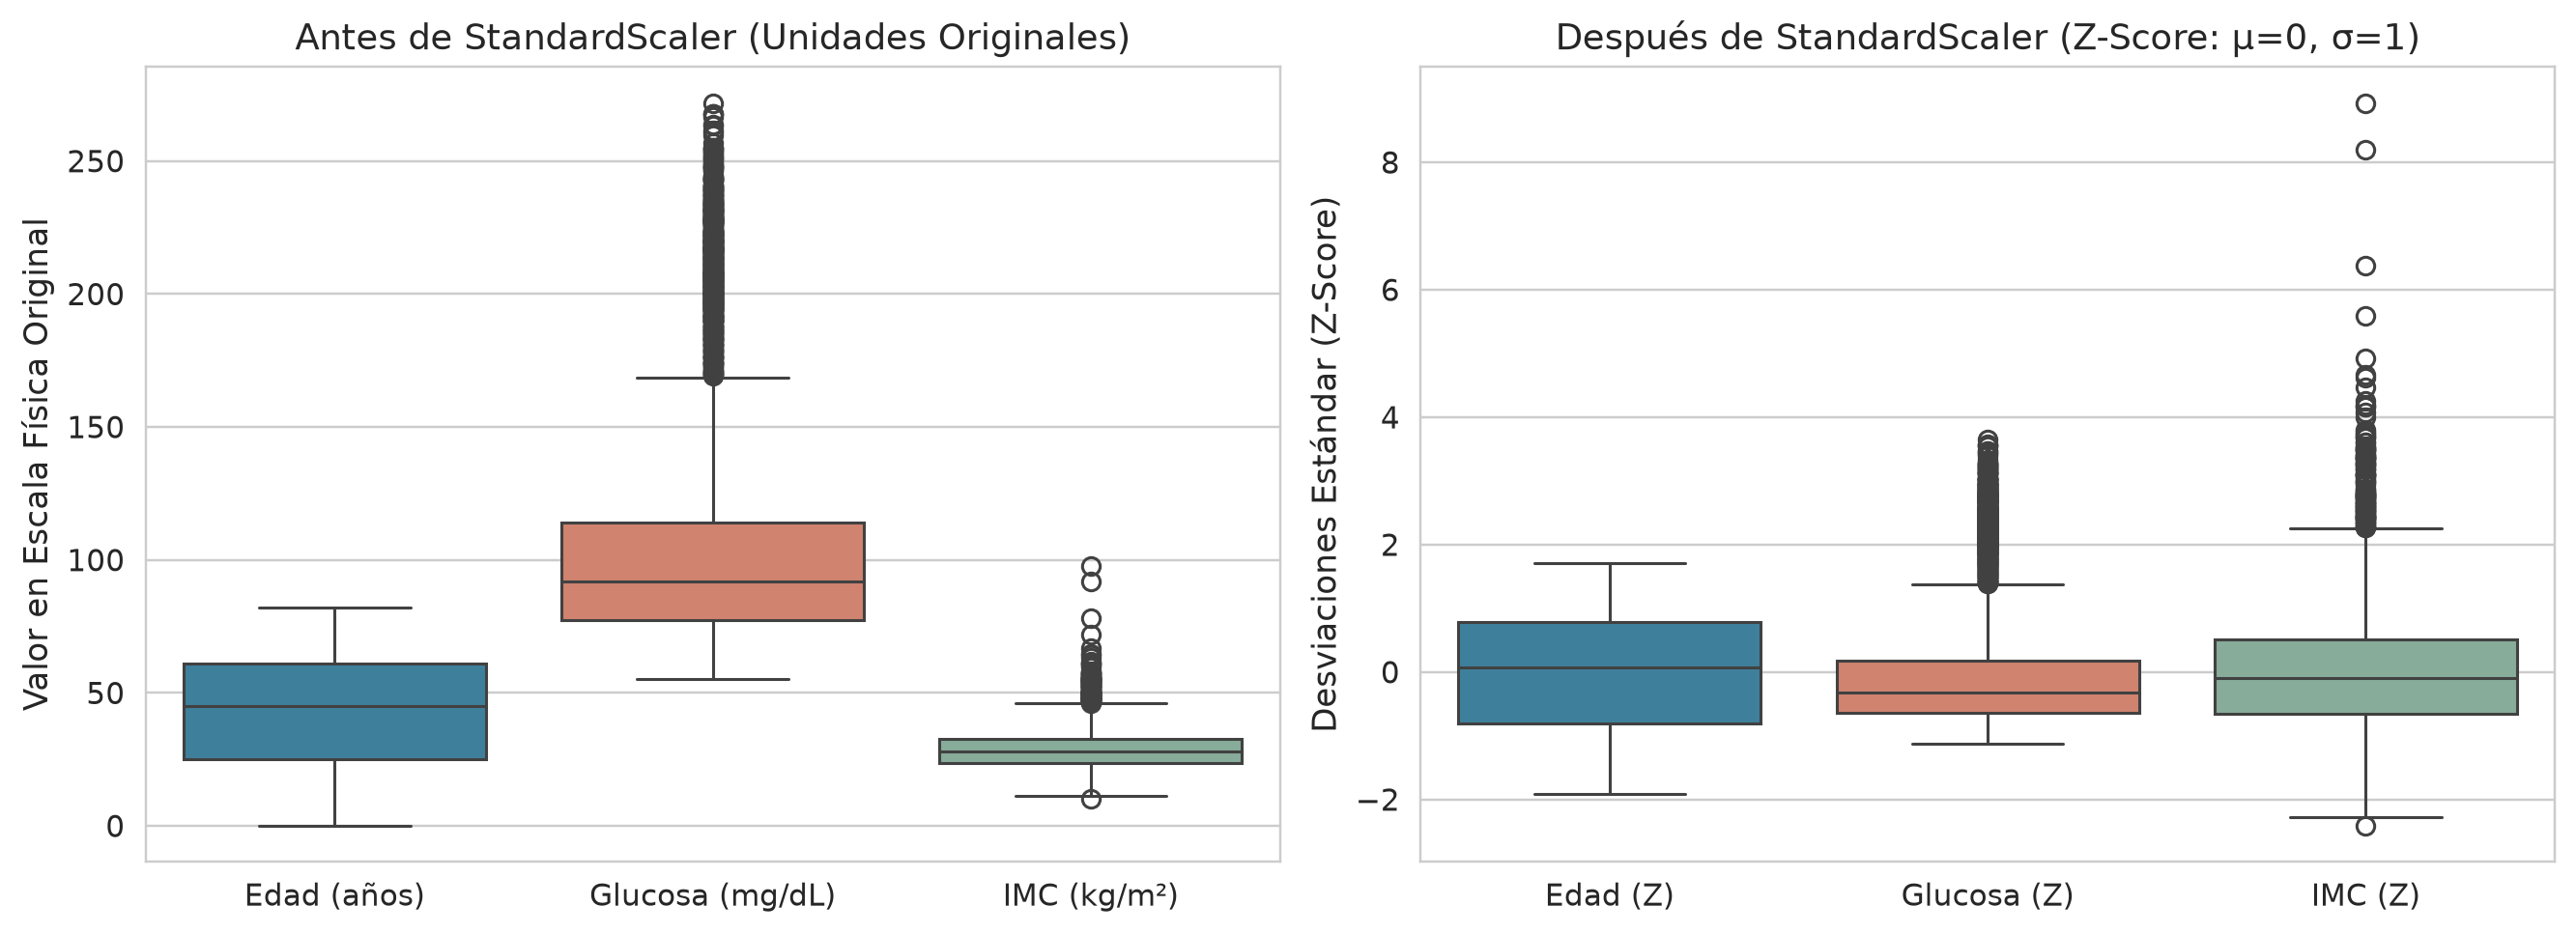
\includegraphics[width=0.96\textwidth]{Imágenes/fig_af3_escalado.png}
    \caption{Comparación de las distribuciones de \texttt{age}, \texttt{avg\_glucose\_level} y \texttt{bmi} antes y después de la normalización con \texttt{StandardScaler}.}
    \label{fig:af3_escalado}
\end{figure}

\subsubsection{Investigación: ¿Por qué K-Means fallaría catastróficamente sin escalar los datos?}
La distancia euclidiana al cuadrado entre dos pacientes $\mathbf{x}_i$ y $\mathbf{x}_m$ es aditiva sobre las tres dimensiones:
\begin{equation}
    d^2(\mathbf{x}_i, \mathbf{x}_m) = (x_{i,\text{edad}} - x_{m,\text{edad}})^2 + (x_{i,\text{glucosa}} - x_{m,\text{glucosa}})^2 + (x_{i,\text{bmi}} - x_{m,\text{bmi}})^2.
\end{equation}
Como demuestra la Tabla~\ref{tab:stats_escalado}, la varianza sin escalar de \texttt{avg\_glucose\_level} ($2,050.60\text{ mg}^2/\text{dL}^2$) es \textbf{$4.01$ veces mayor que la varianza de la edad} ($511.33$) y \textbf{$34.59$ veces mayor que la varianza del IMC} ($59.28$). En consecuencia:
\begin{enumerate}
    \item \textbf{Dominancia numérica de la glucosa:} una variación clínica moderada de $100\text{ mg/dL}$ en glucosa aporta $100^2 = 10,000$ a la suma cuadrática, mientras que una diferencia crítica de $20\text{ kg/m}^2$ en el IMC (la diferencia entre normopeso y obesidad mórbida) aporta únicamente $20^2 = 400$ ($25$ veces menos peso en el criterio de partición).
    \item \textbf{Deformación de las celdas de Voronoi:} K-Means asume clústeres esféricos de varianza isotrópica en todas las direcciones. Sin escalar, el algoritmo particionaría el espacio casi exclusivamente en franjas horizontales de glucosa, ignorando por completo la información del IMC y subestimando la edad. Al estandarizar a media $\mu = 0$ y varianza $\sigma^2 = 1$, las tres variables clínicas contribuyen con pesos geométricos equitativos.
\end{enumerate}

\subsection{Sección 2: Búsqueda del Número Óptimo de Clústeres (Método del Codo y Silueta)}

Para determinar objetivamente el número óptimo de perfiles $k$, se entrenaron modelos \texttt{KMeans} con inicialización \texttt{k-means++} \cite{Arthur2007} (\texttt{n\_init=10, random\_state=42}) variando $k \in \{1, 2, \dots, 10\}$. Para cada configuración se registró la inercia intra-clúster $WCSS(k)$ y, para $k \ge 2$, el \textbf{Coeficiente de Silueta promedio} \cite{Rousseeuw1987}:
\begin{equation}
    s(i) = \frac{b(i) - a(i)}{\max\{a(i),\, b(i)\}} \in [-1, 1],
\end{equation}
donde $a(i)$ es la distancia media del paciente $i$ a los demás miembros de su propio clúster (cohesión) y $b(i)$ es la distancia media hacia los miembros del clúster vecino más próximo (separación).

\begin{table}[H]
    \centering
    \caption{Evolución de la Inercia (WCSS) y del Coeficiente de Silueta para $k \in [1, 10]$.}
    \label{tab:codo_silueta}
    \begin{tabular}{cccc}
        \toprule
        \textbf{Clústeres ($k$)} & \textbf{Inercia (WCSS)} & \textbf{Reducción Marginal (\%)} & \textbf{Coeficiente de Silueta} \\
        \midrule
        1  & 15,330.00 & ---     & --- (No definido para $k=1$) \\
        2  & 10,386.75 & 32.25\% & 0.3002 \\
        3  & 6,813.68  & 34.40\% & 0.3714 \\
        \textbf{4} & \textbf{5,140.29} & \textbf{24.56\%} & \textbf{0.3727 (Máximo Global)} \\
        5  & 4,387.45  & 14.65\% & 0.3231 \\
        6  & 3,979.98  & 9.29\%  & 0.3117 \\
        7  & 3,610.54  & 9.28\%  & 0.2828 \\
        8  & 3,304.18  & 8.49\%  & 0.2835 \\
        9  & 3,041.88  & 7.94\%  & 0.2899 \\
        10 & 2,807.40  & 7.71\%  & 0.2781 \\
        \bottomrule
    \end{tabular}
\end{table}

\begin{figure}[H]
    \centering
    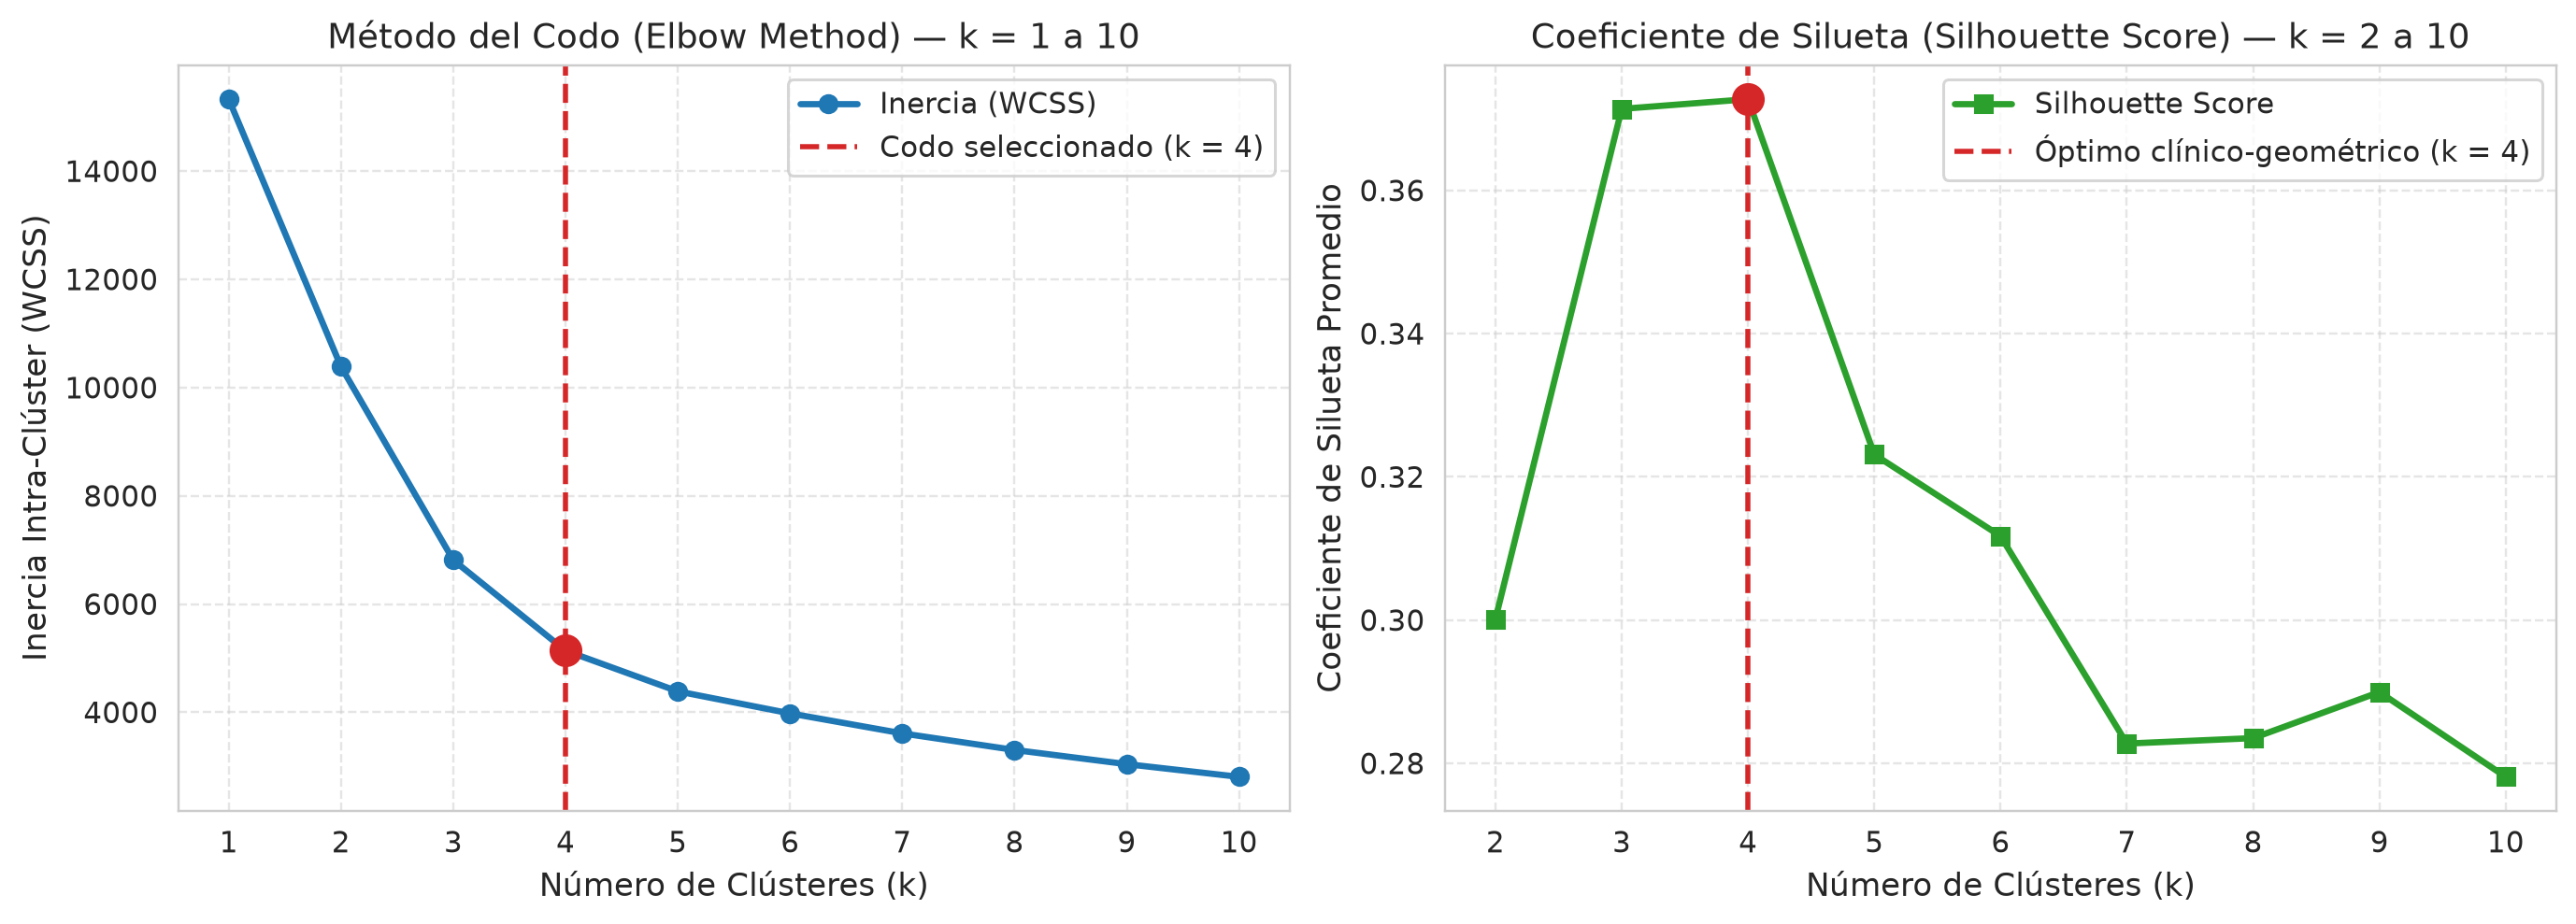
\includegraphics[width=0.98\textwidth]{Imágenes/fig_af3_codo_silueta.png}
    \caption{Determinación matemática de $k$: Método del Codo (izquierda) y Coeficiente de Silueta (derecha), coincidiendo ambos criterios en el óptimo $k = 4$.}
    \label{fig:af3_codo_silueta}
\end{figure}

Tanto la Tabla~\ref{tab:codo_silueta} como la Figura~\ref{fig:af3_codo_silueta} demuestran una convergencia exacta entre ambos criterios matemáticos en \textbf{$k = 4$ clústeres}:
\begin{itemize}
    \item En la curva de inercia, las mayores reducciones porcentuales ocurren al pasar de $k=1 \to 2$ ($32.25\%$), $k=2 \to 3$ ($34.40\%$) y $k=3 \to 4$ ($24.56\%$). A partir de $k=5$, la ganancia cae por debajo del $15\%$ y se vuelve lineal.
    \item En la curva de silueta, \textbf{$k = 4$ alcanza el máximo global absoluto ($0.3727$)}, superando a $k=3$ ($0.3714$) y cayendo abruptamente en $k=5$ ($0.3231$) debido a la sobre-fragmentación artificial de pacientes normoglucémicos.
\end{itemize}

\subsection{Sección 3: Entrenamiento del Modelo Final y Visualización de Centroides}

Con $k = 4$ fijado como valor óptimo, se ajustó el modelo final \texttt{KMeans(n\_clusters=4, random\_state=42, n\_init=10)}. La Tabla~\ref{tab:centroides} reporta las coordenadas exactas de los cuatro centroides tanto en unidades clínicas originales (obtenidas mediante \texttt{scaler.inverse\_transform}) como en puntuaciones estandarizadas $Z$.

\begin{table}[H]
    \centering
    \caption{Coordenadas de los centroides descubiertos por K-Means ($k = 4$) e interpretación médica del perfil.}
    \label{tab:centroides}
    \begin{tabular}{lccc|ccc|cc}
        \toprule
        & \multicolumn{3}{c|}{\textbf{Unidades Clínicas Reales}} & \multicolumn{3}{c|}{\textbf{Espacio Estandarizado ($Z$)}} & \multicolumn{2}{c}{\textbf{Tamaño}} \\
        \textbf{Clúster} & \textbf{Edad} & \textbf{Glucosa} & \textbf{IMC} & $Z_{\text{edad}}$ & $Z_{\text{gluc}}$ & $Z_{\text{bmi}}$ & $n$ & \textbf{\%} \\
        \midrule
        \textbf{Clúster 0} (Adulto Mayor Normoglucémico) & 60.03 & 89.54 & 27.74 & $+0.74$ & $-0.37$ & $-0.15$ & 1,877 & 36.73\% \\
        \textbf{Clúster 1} (Adulto Obesidad Normoglucémica) & 41.52 & 90.32 & \textbf{39.03} & $-0.08$ & $-0.35$ & $\mathbf{+1.32}$ & 922 & 18.04\% \\
        \textbf{Clúster 2} (Joven / Pediátrico Saludable) & 17.89 & 92.67 & 22.81 & $-1.12$ & $-0.30$ & $-0.79$ & 1,639 & 32.07\% \\
        \textbf{Clúster 3} (Adulto Mayor Hiperglucémico) & \textbf{60.54} & \textbf{207.30} & \textbf{32.75} & $\mathbf{+0.77}$ & $\mathbf{+2.23}$ & $+0.51$ & 672 & 13.15\% \\
        \bottomrule
    \end{tabular}
\end{table}

\begin{figure}[H]
    \centering
    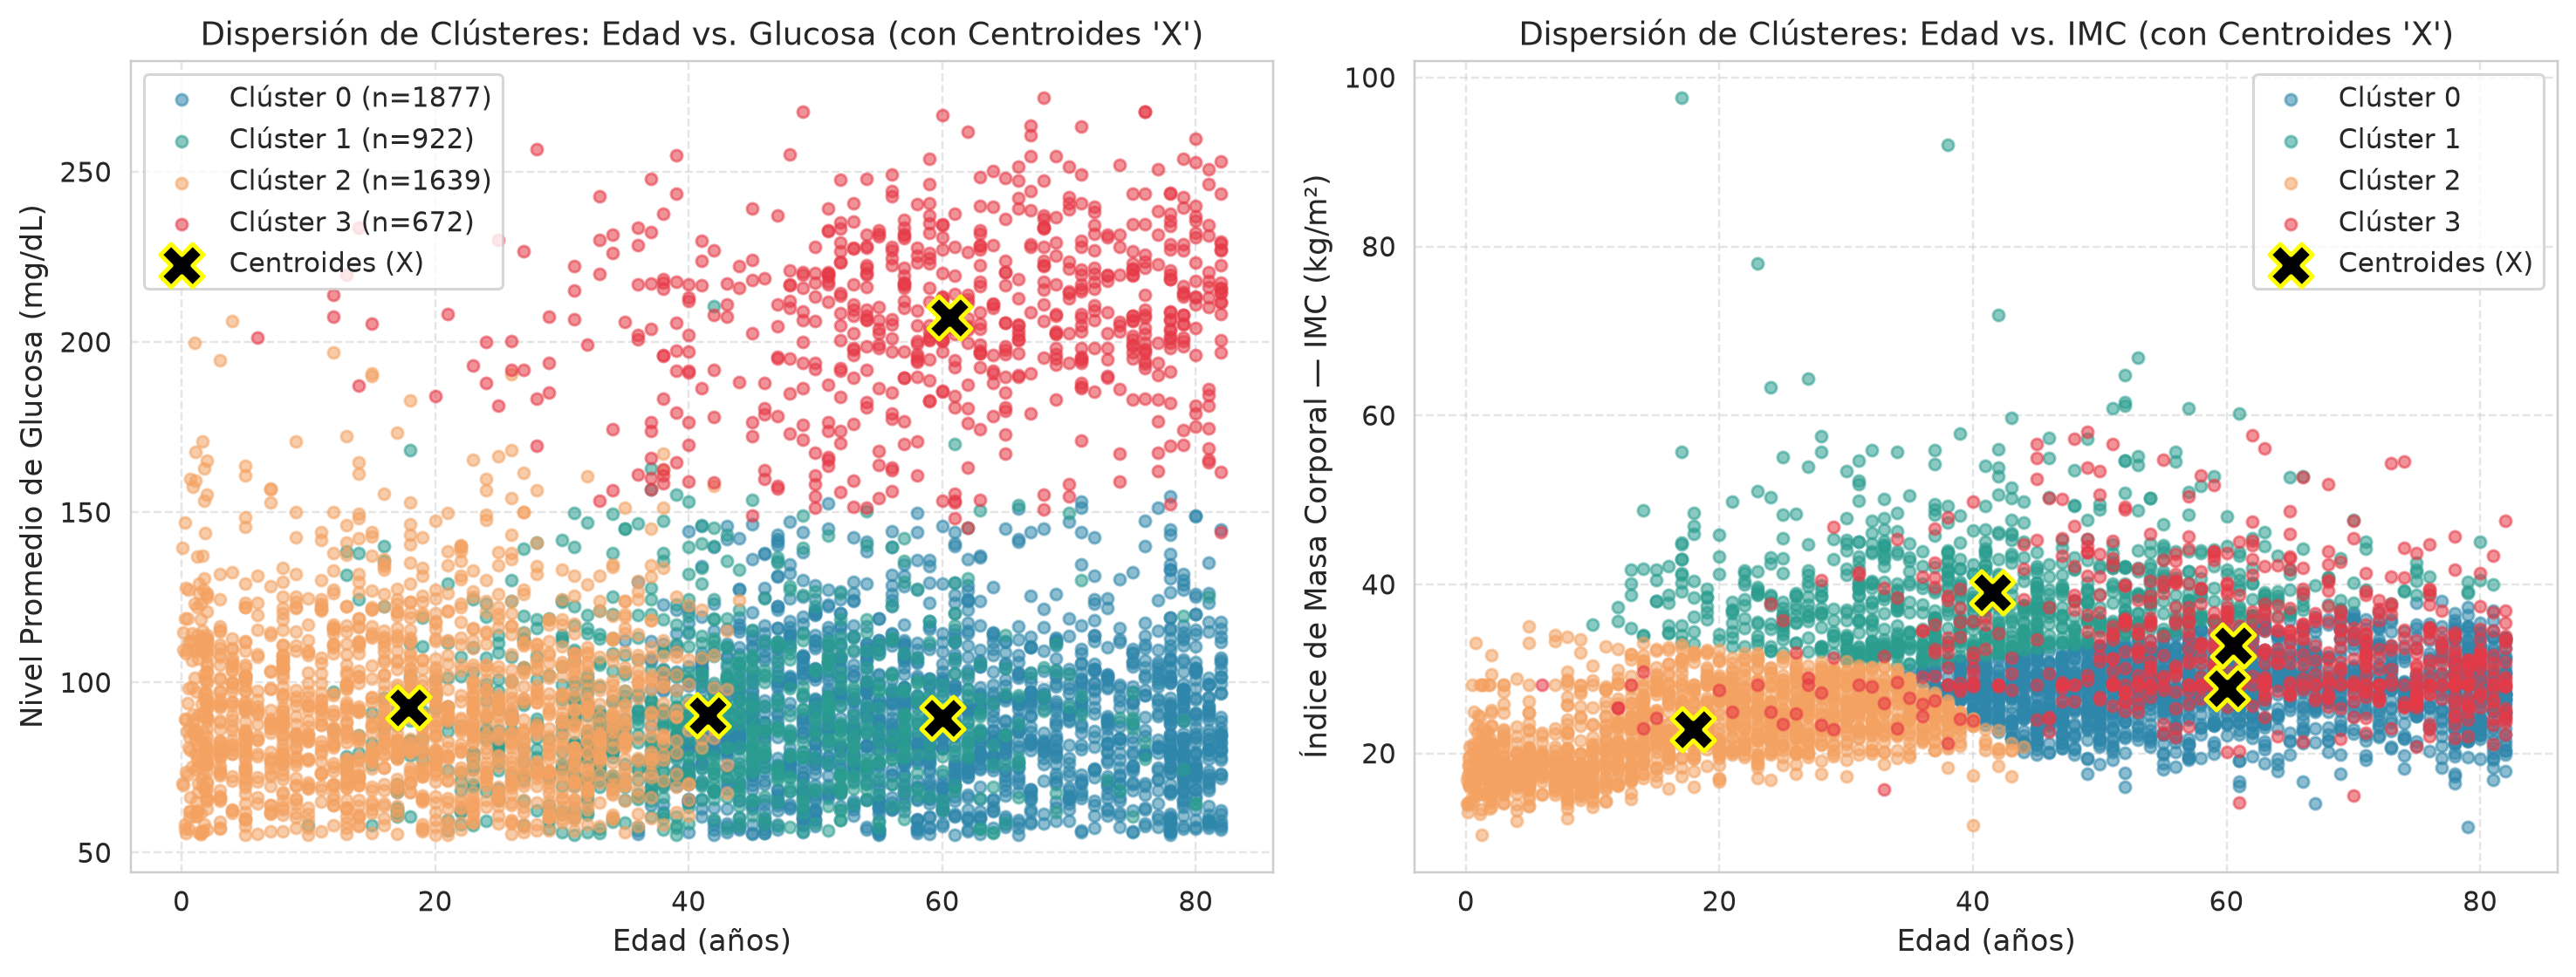
\includegraphics[width=0.98\textwidth]{Imágenes/fig_af3_dispersion_centroides.png}
    \caption{Gráficos de dispersión de pacientes coloreados por clúster asignado: Edad vs.\ Glucosa (izquierda) y Edad vs.\ IMC (derecha), marcando con una \textbf{«X»} la posición de los cuatro centroides.}
    \label{fig:af3_dispersion}
\end{figure}

\begin{figure}[H]
    \centering
    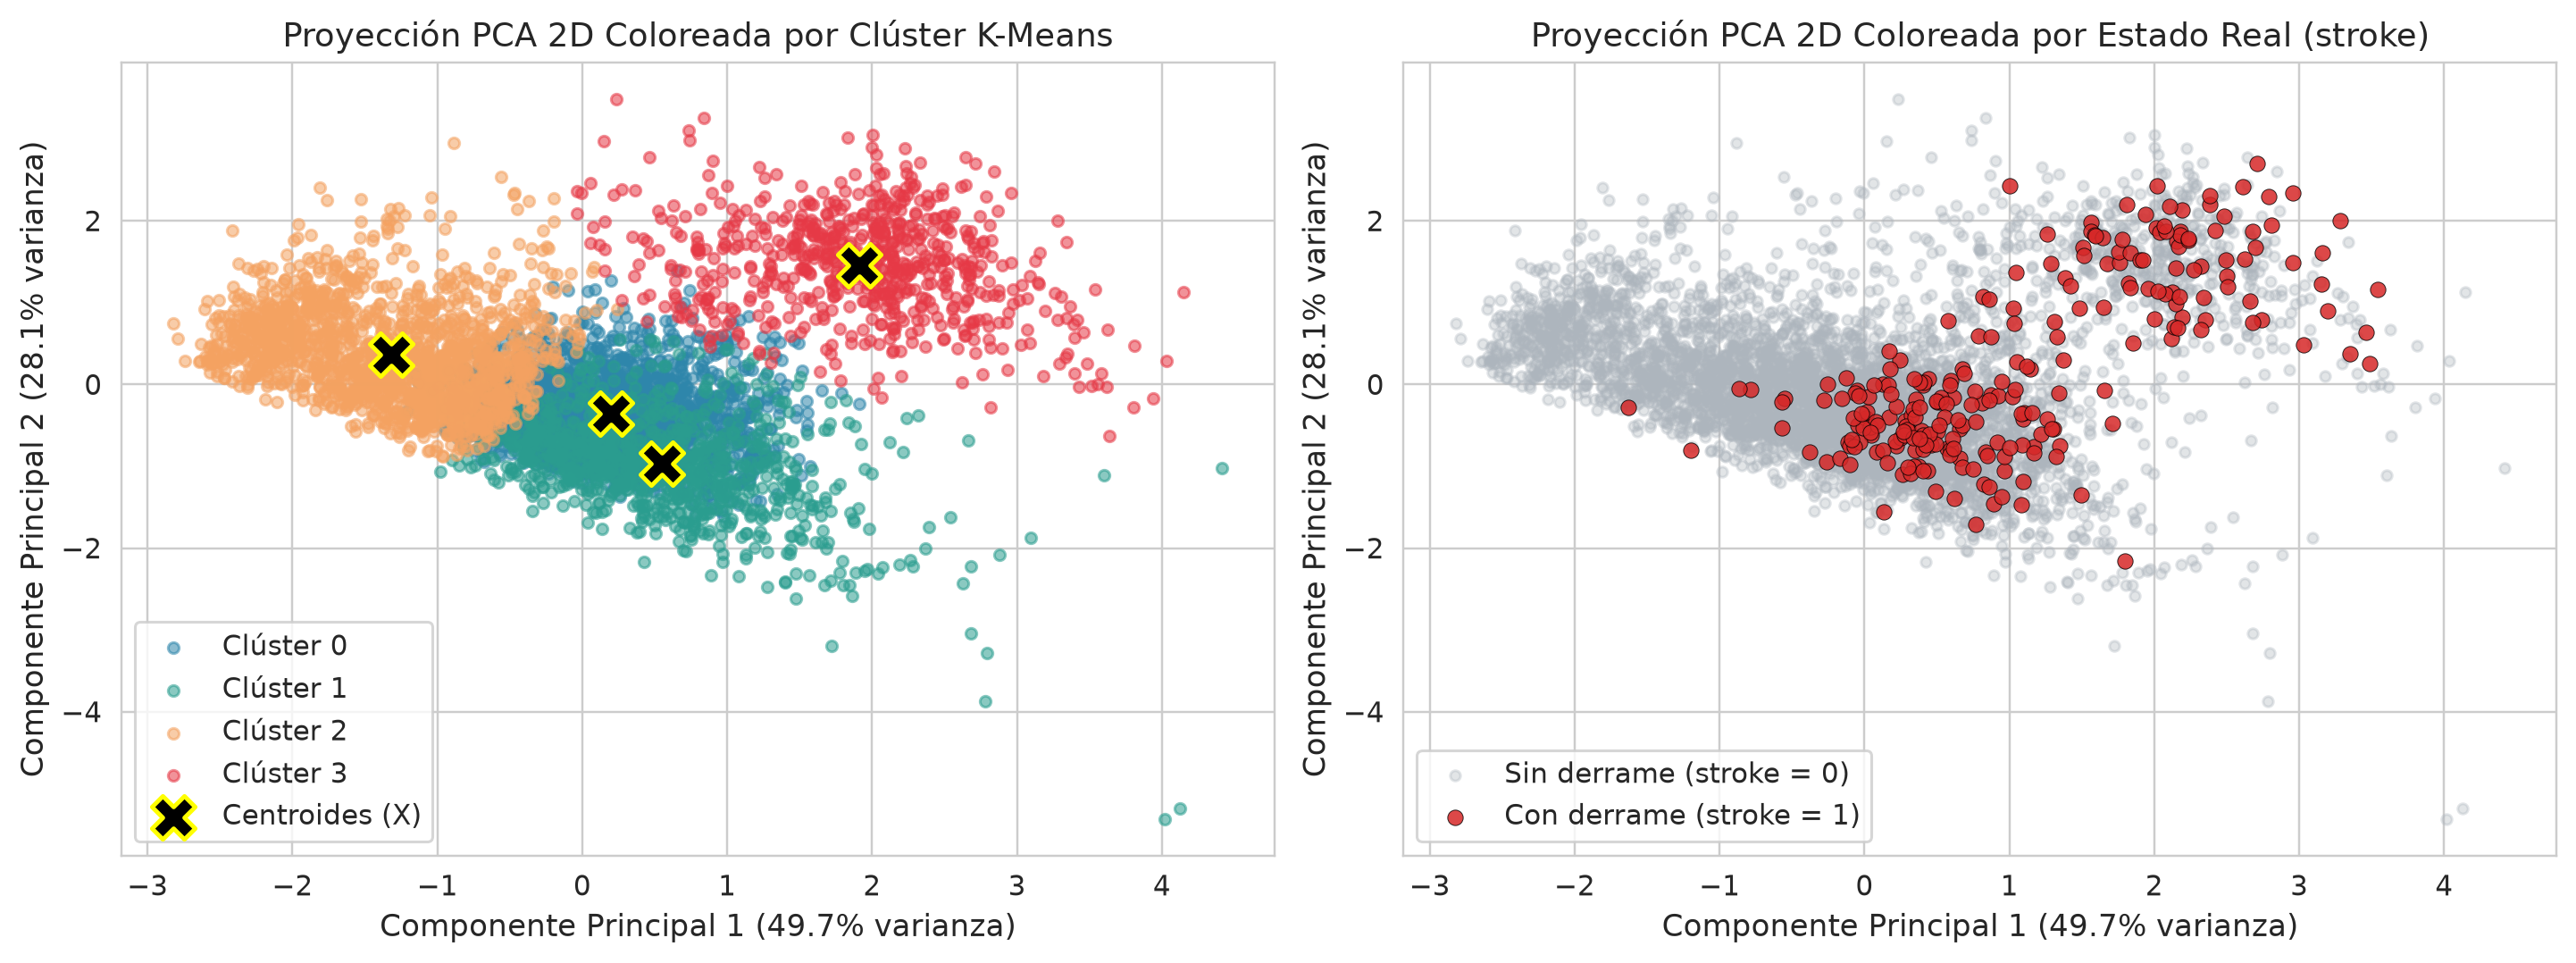
\includegraphics[width=0.98\textwidth]{Imágenes/fig_af3_pca_clusters.png}
    \caption{Proyección bidimensional mediante Análisis de Componentes Principales (PCA, $77.88\%$ de varianza explicada): clústeres y centroides «X» (izquierda) frente a la distribución real de casos con derrame cerebral (derecha).}
    \label{fig:af3_pca}
\end{figure}

La Figura~\ref{fig:af3_dispersion} ilustra con claridad la partición geométrica lograda en el espacio clínico:
\begin{itemize}
    \item En el plano \textbf{Edad vs.\ Glucosa} (panel izquierdo), el \textbf{Clúster 3} (puntos rojos, centroide «X» en $60.54\text{ años}$ y $207.30\text{ mg/dL}$) aísla nítidamente el estrato superior de pacientes con hiperglucemia severa ($>150\text{ mg/dL}$), mientras que los tres clústeres restantes dividen la banda normoglucémica a lo largo del eje de edad ($17.89$, $41.52$ y $60.03\text{ años}$).
    \item En el plano \textbf{Edad vs.\ IMC} (panel derecho), se observa cómo el \textbf{Clúster 1} (puntos verde azulado, centroide «X» en $39.03\text{ kg/m}^2$) separa a los adultos de mediana edad con obesidad grado II/III de los adultos mayores con sobrepeso ligero del \textbf{Clúster 0} ($27.74\text{ kg/m}^2$).
\end{itemize}

\subsection{Sección 4: Validación Cruzada Externa con la Variable Real \texttt{stroke}}

Una vez concluido el agrupamiento no supervisado, se reincorporó la etiqueta reservada \texttt{stroke} al DataFrame con las asignaciones de clúster para construir la tabla de contingencia (\texttt{pd.crosstab}) presentada en la Tabla~\ref{tab:crosstab_stroke} y graficada en la Figura~\ref{fig:af3_crosstab}.

\begin{table}[H]
    \centering
    \caption{Tabla cruzada (\texttt{pd.crosstab}) entre los clústeres descubiertos a ciegas por K-Means y la ocurrencia real de derrame cerebral (\texttt{stroke}).}
    \label{tab:crosstab_stroke}
    \begin{tabular}{lccccc}
        \toprule
        \textbf{Clúster Descubierto} & \textbf{Sin Derrame ($0$)} & \textbf{Con Derrame ($1$)} & \textbf{Total ($n$)} & \textbf{Prevalencia Intra-Clúster} & \textbf{\% del Total de Derrames} \\
        \midrule
        \textbf{Clúster 0} (Adulto Mayor Normoglucémico) & 1,736 & 141 & 1,877 & 7.51\% ($1.54\times$ basal) & \textbf{56.63\%} \\
        \textbf{Clúster 1} (Adulto Obesidad Normoglucémica) & 907 & 15 & 922 & 1.63\% ($0.33\times$ basal) & 6.02\% \\
        \textbf{Clúster 2} (Joven / Pediátrico Saludable) & 1,635 & 4 & 1,639 & 0.24\% ($0.05\times$ basal) & 1.61\% \\
        \textbf{Clúster 3} (Adulto Mayor Hiperglucémico) & 583 & 89 & 672 & \textbf{13.24\% ($2.72\times$ basal)} & \textbf{35.74\%} \\
        \midrule
        \textbf{Total Global} & \textbf{4,861} & \textbf{249} & \textbf{5,110} & \textbf{4.87\% (Tasa Basal)} & \textbf{100.00\%} \\
        \bottomrule
    \end{tabular}
\end{table}

\begin{figure}[H]
    \centering
    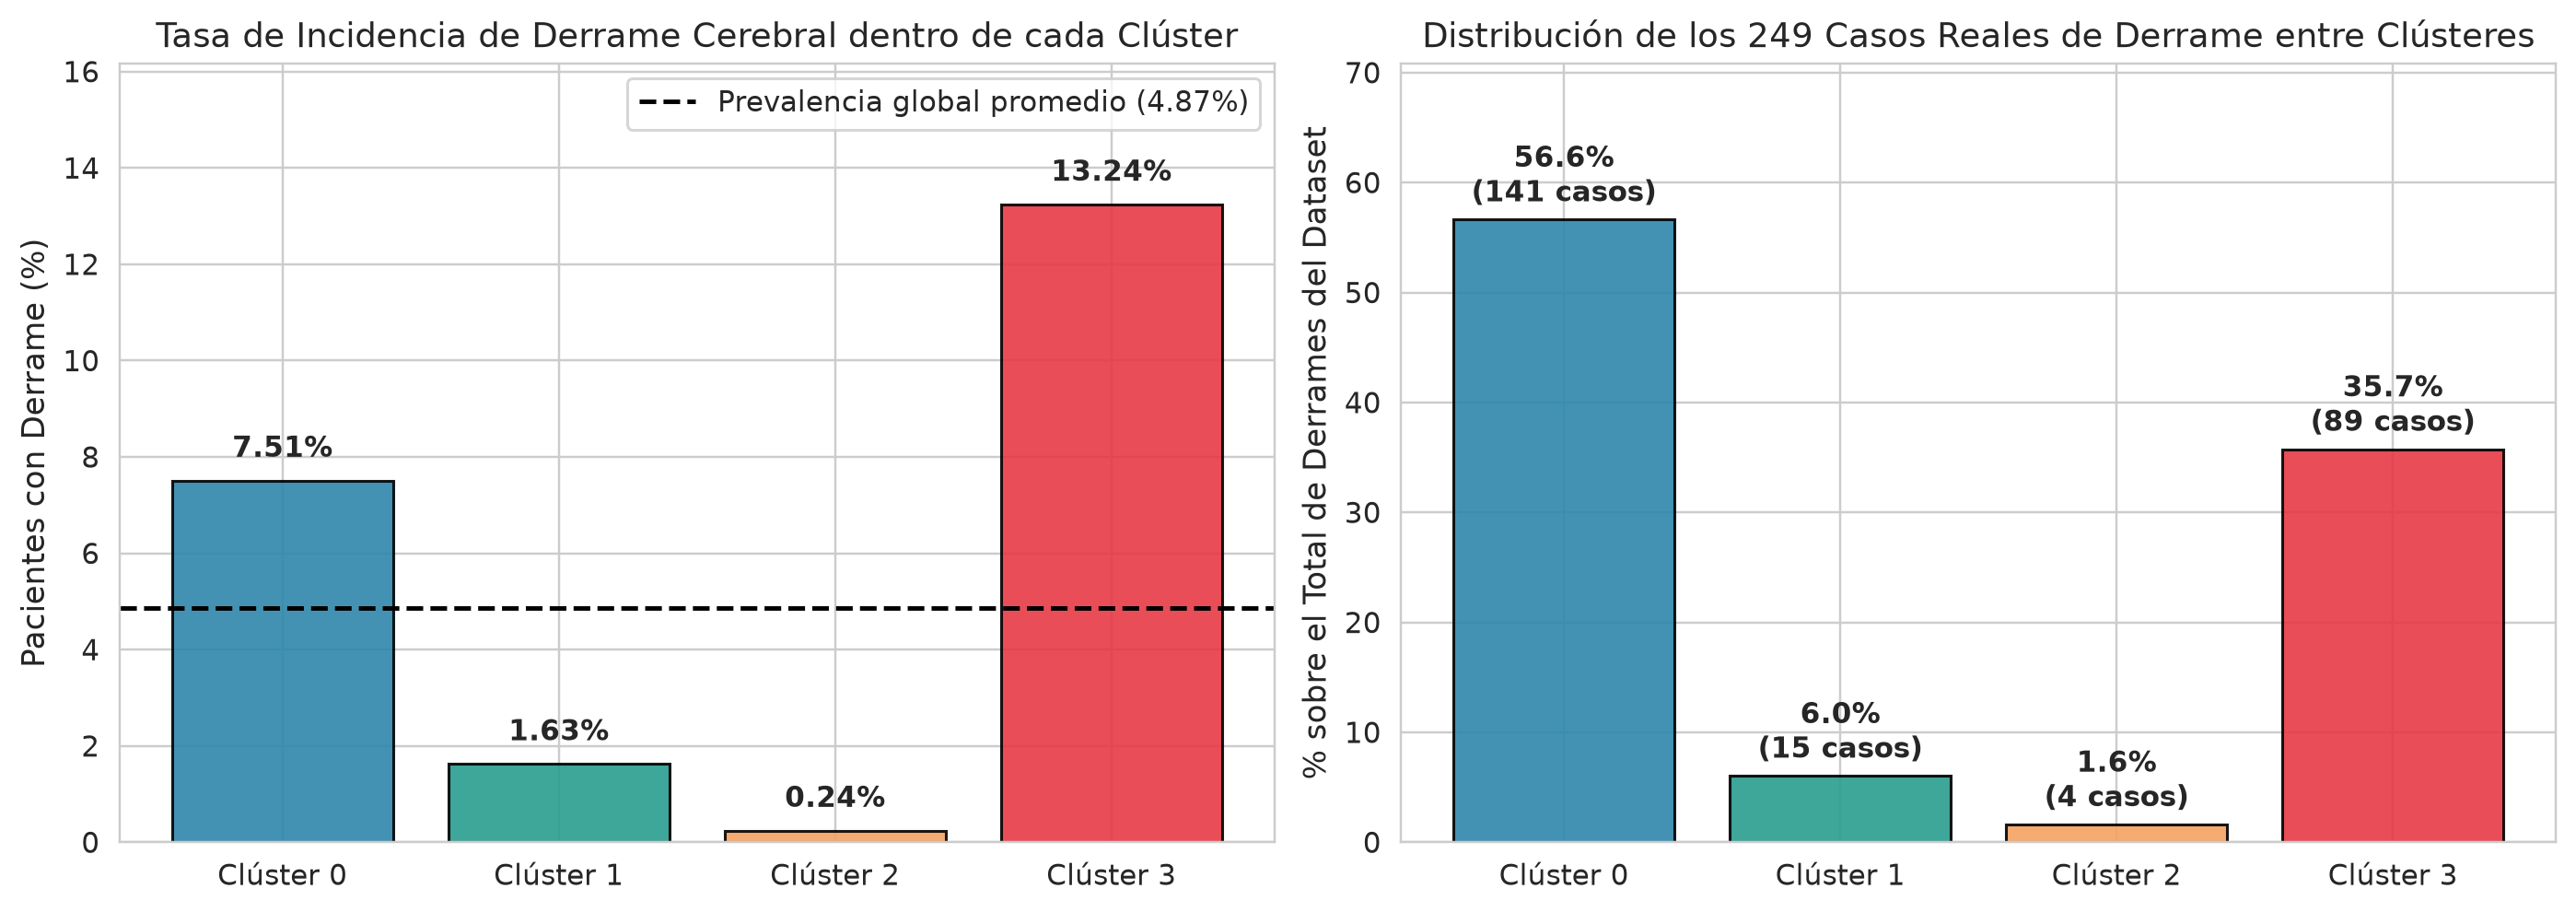
\includegraphics[width=0.98\textwidth]{Imágenes/fig_af3_crosstab_stroke.png}
    \caption{Validación cruzada externa: tasa de incidencia de derrame cerebral dentro de cada clúster respecto al promedio global del $4.87\%$ (izquierda) y distribución porcentual de los 249 casos reales de derrame entre los cuatro clústeres (derecha).}
    \label{fig:af3_crosstab}
\end{figure}

\subsubsection{Respuesta a la Pregunta Final de Análisis}
\begin{enumerate}
    \item \textbf{¿Cuál de los clústeres formados concentra el mayor porcentaje de casos reales de derrame cerebral?}
    \begin{itemize}
        \item \textbf{Mayor prevalencia o riesgo relativo intra-clúster:} El \textbf{Clúster 3} (\textit{Adulto Mayor con Hiperglucemia Severa}, edad media $60.54\text{ años}$, glucosa media $207.30\text{ mg/dL}$ e IMC $32.75\text{ kg/m}^2$) presenta la tasa más alta de enfermedad con un \textbf{13.24\%} de sus pacientes habiendo sufrido un derrame cerebral ($89$ de $672$). Esta incidencia es \textbf{$2.72$ veces superior} a la tasa basal de la población ($4.87\%$) y \textbf{$54.3$ veces superior} a la del Clúster 2 ($0.24\%$).
        \item \textbf{Mayor volumen sobre el total de los 249 derrames:} El \textbf{Clúster 0} (\textit{Adulto Mayor Normoglucémico}, edad media $60.03\text{ años}$, $n = 1,877$) agrupa el \textbf{56.63\%} ($141/249$) de todos los eventos cerebrovasculares del estudio (con una prevalencia interna del $7.51\%$), seguido directamente por el \textbf{Clúster 3} con el \textbf{35.74\%} ($89/249$).
    \end{itemize}
    \item \textbf{¿El algoritmo de clustering fue capaz de aislar un grupo de alto riesgo médico sin haber visto nunca la etiqueta \texttt{stroke}?}
    \textbf{Sí, de manera altamente efectiva.} A pesar de operar completamente a ciegas respecto al diagnóstico de derrame cerebral, K-Means identificó en el \textbf{Clúster 3} la intersección fisiológica de mayor peligro clínico (senescencia vascular combinada con diabetes/hiperglucemia descontrolada y sobrepeso), concentrando en apenas el $13.15\%$ de la población más de una tercera parte ($35.74\%$) de todos los derrames cerebrales. Más aún, al considerar conjuntamente los dos perfiles geriátricos descubiertos de forma no supervisada (\textbf{Clúster 3 + Clúster 0}), el modelo aísla el \textbf{92.37\% ($230$ de $249$) de todos los casos reales de accidente cerebrovascular}.
\end{enumerate}

\subsection{Enlace al Repositorio de GitHub con la Solución Ejecutable}

La libreta interactiva de Python con todo el código, gráficas y validaciones de esta Actividad Fundamental 3 se encuentra alojada en el repositorio oficial del equipo en GitHub:
\begin{itemize}
    \item \textbf{Repositorio GitHub:} \url{https://github.com/Xraight/FIME-Machine-Learning-}
    \item \textbf{Ruta de la libreta AF3:} \texttt{AF3/AF3.ipynb}
    \item \textbf{Abrir directamente en Google Colab:} \url{https://colab.research.google.com/github/Xraight/FIME-Machine-Learning-/blob/main/AF3/AF3.ipynb}
\end{itemize}

\section{Conclusión}

El desarrollo de la Actividad Fundamental 3 permitió comprobar experimentalmente el valor clínico y matemático del aprendizaje no supervisado basado en particiones:
\begin{enumerate}
    \item \textbf{Necesidad crítica de estandarización:} Se demostró analítica y empíricamente que, debido a que la varianza de la glucosa ($2,050.60$) supera en $34.6\times$ a la del IMC ($59.28$) y en $4.0\times$ a la de la edad ($511.33$), omitir \texttt{StandardScaler} haría que la métrica euclidiana de K-Means colapsara sobre una sola dimensión fisiológica.
    \item \textbf{Determinación objetiva del número de perfiles:} La combinación del Método del Codo y el Coeficiente de Silueta identificó sin ambigüedad un óptimo en $k = 4$ clústeres (máximo global de silueta $= 0.3727$, inercia $= 5,140.29$), evitando decisiones arbitrarias.
    \item \textbf{Descubrimiento emergente de riesgo cerebrovascular:} La validación cruzada contra la etiqueta oculta \texttt{stroke} demostró que la estructura geométrica natural de las variables continuas (\texttt{age}, \texttt{avg\_glucose\_level}, \texttt{bmi}) refleja fielmente la fisiopatología del accidente cerebrovascular, aislando en el Clúster 3 una tasa de incidencia de $13.24\%$ ($2.72\times$ el riesgo basal) y capturando entre los dos clústeres de adultos mayores el $92.37\%$ de todos los derrames del conjunto de datos.
\end{enumerate}

	
	\newpage
	\nocite{*}
	\bibliographystyle{apalike}
	\bibliography{bibliografia.bib}
	
	\centering\small
	\bigskip
	Las imágenes utilizadas en este documento son propiedad de sus respectivos autores y se incluyen únicamente con fines académicos.
	
\end{document}
